\documentclass[letterpaper]{article} % DO NOT CHANGE THIS
\usepackage{aaai2027}  % DO NOT CHANGE THIS
\usepackage[hyphens]{url}  % DO NOT CHANGE THIS
\usepackage{graphicx} % DO NOT CHANGE THIS
\urlstyle{rm} % DO NOT CHANGE THIS
\def\UrlFont{\rm}  % DO NOT CHANGE THIS
\usepackage{natbib}  % DO NOT CHANGE THIS AND DO NOT ADD ANY OPTIONS TO IT
\usepackage{caption} % DO NOT CHANGE THIS AND DO NOT ADD ANY OPTIONS TO IT
\frenchspacing  % DO NOT CHANGE THIS
\usepackage{booktabs}
\usepackage{amsfonts}
\usepackage{amsmath}
\graphicspath{{../figs/}}
\usepackage{xr}
\externaldocument{supplement}
\pdfinfo{
/TemplateVersion (2027.1)
}
\setcounter{secnumdepth}{0}

\title{Black--Scholes for the Land:\\ Modelling Savannah Response to Rain as a Dynamic World Model}
\author{
    Tom Pitts
}
\affiliations{
    AFFILIATION TO CONFIRM\\
    tom.d.pitts@gmail.com
}

\begin{document}
\maketitle

\begin{abstract}
Carbon credits, offsets and index insurance rest on counterfactuals: what the land would have done under the same weather without management, or what a bad season cost. Current baselines fail in two ways: some ignore rain, others condition on rain linearly and annually. But the true response lags the rain, depends on hidden state such as moisture from other sources, and responds differently from pixel to pixel. Focussing on grassland pasture and rainfall specifically as a proof of concept, we fit a temporal world model of MODIS greenness conditioned on CHIRPS rain over two $45\times45$\,km regions in Laikipia, Kenya: a transition density map for greenness given recent and current rainfall. We use it, conceptually, as Black--Scholes is used. Inverting the model on observed greenness it yields an implied residual, everything the land did that the rain does not explain. Two capabilities drop out of this solution: 1) attribution, what the land did beyond the rain; 2) sensitivities, derivatives of the rollout with respect to rain and state, close analogues of the Greeks. On Laikipia test sites, our learned model recovers three-month greenness with $23\%$ less error than a history-only baseline and $13\%$ less than the best hand-written model on unseen years. In the 2022 drought, the land ended $0.17$ NDVI below normal; the rain that failed explains roughly half of that, and under normal rain with the same residual it would still have ended $0.10$ below. $\Delta$, the derivative of greenness with respect to rain, is computed at every pixel and averages $0.075$ NDVI per extra $100$\,mm of rain. A $\Delta$ at every pixel is an exposure to rain that can be hedged, allowing efficient pricing of contracts and accurate attribution. The deep learning approach we describe here could furthermore be used with other data inputs beyond rain to derive yet more finegrained attribution and sensitivities.
\end{abstract}

\section{Approach}
Various methodologies exist to measure the carbon capture attributable to sustainable grassland management practices, such as rotation of grazing animals, replanting strategies, and backburning. The Northern Kenya Rangelands Carbon Project, the world's largest soil carbon removal project, earns one credit per tonne of CO$_2$ stored in soil above a baseline set by VM0032, a pioneering grazing methodology \citep{vm0032,verra2023}. However, that baseline was contested enough for Verra to suspend issuance for eight months in 2023 \citep{verra2023,si2023}. Its baseline model, SNAP \citep{ritchie2014,nkgcp_pd2016}, uses only mean annual rainfall, rather than an input such as CHIRPS 16-day periodic rainfall \citep{nkcp} or even seasonal rain records. Elsewhere, livestock index insurance in the same counties pays on seasonal NDVI against the pixel's own history \citep{ibli}. For maximum efficiency, the insurer ideally would want to quantify forage lost to drought, rather than management decisions such as overgrazing. Both payments would benefit from a clean split between what the land did because of the climate and what it did because of everything else, and to the best of our knowledge, no current operational baseline makes that split cleanly. The model we propose makes that split with climate as its conditioning input. In this work we demonstrate the concept with rainfall alone, the key climate driver in these rangelands, estimating the specific terrain response from data as a transition density $p_\theta(a_{t+1}\mid a_t, w_t, r_{t+1})$ for the greenness anomaly $a$ given a rain-memory state $w$ and rainfall $r$.

A Black-Scholes formula (BSF) model \citep{bs} is fed observables such as current stock price, strike price, and used to derive a parameter value -- implied volatility -- which cannot be observed directly but is implied by the market's current pricing of options. In our model the observables are the total state and the rain that fell, and the model is inverted on observed greenness. What comes out is the residual i.e. what the land did beyond what the rain by itself explains. Furthermore, specific values can also be plugged back in to the model. The model can be re-run with the residual held fixed and the rain replaced, and it returns the land under that other rain with everything else as it was. Derivatives come by automatic differentiation, as the Greeks come from the BSF.

\paragraph{Residual} The residual between modelled and observed includes everything not in the model. That includes grazing, clearing and fire, the management and disturbance signal itself, but also climate effects other than rain (temperature, evaporative demand) that this demonstration does not condition on, error in the CHIRPS rainfall product, error in the fitted response, and satellite noise. We assume error in CHIRPS and noise are statistically constant over a sufficiently large dataset.

\section{Related Work}
Separating climate from land use in vegetation records is an old problem. Residual trend analysis regresses annual or growing-season NDVI on accumulated rainfall and reads trends in the residual as human-induced degradation \citep{evans2004,wessels2007}; later variants find breakpoints in the residual trend \citep{burrell2017}, and vegetation sensitivity indices add a one-month memory term \citep{seddon2016}. These are linear in their drivers and fitted pixel by pixel at annual or monthly scale. M1 below is a 16-day version; M2 replaces the regression with a learned, state-dependent transition density shared across pixels. In East Africa, NDVI tracks the rain of the current and two preceding months, with a response that flattens in wetter areas \citep{nicholson1990,davenport1993}. Operational drought monitoring and livestock insurance in Kenya score NDVI against the pixel's own history \citep{kogan1990,klisch2016,vrieling2014,ibli}: the history-only baseline M0. Deep temporal models conditioned on weather already predict crop yield \citep{shook2021}; probabilistic deep forecasters and time-series foundation models output predictive densities \citep{salinas2020,rasul2023,ansari2024}, and one has forecast leaf area index zero-shot \citep{zhang2025}. None is built to be inverted on observations or re-run under another driver path.

\section{Setup}
\paragraph{Data} The target $a_t$ is greenness, the normalised difference vegetation index (NDVI) from the MODIS satellite product MOD13Q1 \citep{mod13}, at $250$\,m every 16 days (one composite), 2002--2025, as an anomaly against each pixel's 2003--2018 climatology. The z-score used throughout is this anomaly divided by the pixel's standard deviation for that time of year. The input $r_t$ is rain from CHIRPS \citep{chirps} summed over the same 16-day windows, in units of $100$\,mm. The setting is two $45$\,km regions in Laikipia, Kenya, with rains in March--May and October--December: Box A (development) and Box B (held-out landscape) to its west (Figure~\ref{fig:map}, Appendix). We fit on Box A 2003--2017, early-stop on 2018, and evaluate on Box A 2019--2025, 14 seasons including the 2021--22 drought and 2023 recovery, and on Box B in every year.

\paragraph{Model} Each step sees only the current state, not the series i.e. Markovian. The state is the anomaly $a_t$ and an antecedent-rain index $w_t$, a one-parameter bucket whose memory $\lambda(x)$ depends on the pixel's traits:
\begin{align}
w_{t+1} &= \lambda(x)\,w_t + r_{t+1}, \nonumber\\
a_{t+1} &= a_t + \mu_\theta(a_t, \bar a_t, w_t, r_{t+1}, \phi_{t+1}, x) \nonumber\\
&\quad + \sigma_\theta(\cdot)\,\varepsilon_t,\qquad \varepsilon_t\sim\mathcal N(0,1),
\label{eq:model}
\end{align}
where $t$ indexes 16-day steps, $\bar a_t$ is the $5\times5$ neighbourhood mean of $a_t$, $\phi_{t+1}$ is the seasonal phase (sine and cosine of day of year), and $x$ is three static traits of the pixel: mean NDVI, seasonal amplitude and climatological annual rain. $w_t$ is a decaying sum of past rain that keeps a fraction $\lambda(x)=\mathrm{sigmoid}(c_0+c^\top x)$ each step. $\mu_\theta$ is the expected change in the anomaly and $\sigma_\theta$ its spread, both functions of the same six inputs, so $p_\theta(a_{t+1}\mid\cdot)=\mathcal N(a_t+\mu_\theta,\sigma_\theta^2)$; $\theta$ is one set of weights shared by every pixel. \textbf{M0} uses history alone. \textbf{M1} has $\mu$ and $\log\sigma$ linear in the features. \textbf{M1.5} adds a hand-written S-curve in $w_t+r_{t+1}$, six parameters. \textbf{M2} adds a 64-unit one-hidden-layer network to $\mu$ and $\log\sigma$. All are fitted by full-batch Adam \citep{kingma2015} on the one-step Gaussian log-likelihood of observed transitions.

\paragraph{Residual} Inverting \eqref{eq:model} on an observed transition gives the implied innovation,
\begin{equation}
\hat\varepsilon_t = \frac{a_{t+1} - a_t - \mu_\theta(a_t,\bar a_t,w_t,r_{t+1},\phi_{t+1},x)}{\sigma_\theta(\cdot)},
\label{eq:implied}
\end{equation}
one number per pixel per 16 days, in units of the model's own spread. Accumulated over a season it is the attribution product: $a_{t+h}-F_h$, where $F_h=\mathbb E[a_{t+h}]$ is the mean rollout along the rain that fell, with the model's spread as its interval. The counterfactual re-runs \eqref{eq:model} from the same state along another rain path $r'$ with $\hat\varepsilon$ held fixed:
\begin{align}
\tilde a_{t+1} &= \tilde a_t + \mu_\theta(\tilde a_t,\bar{\tilde a}_t,\tilde w_t,r'_{t+1},\phi_{t+1},x) \nonumber\\
&\quad + \sigma_\theta(\cdot)\,\hat\varepsilon_t, \nonumber\\
\tilde w_{t+1} &= \lambda(x)\,\tilde w_t + r'_{t+1},\qquad \tilde a_t = a_t.
\label{eq:cf}
\end{align}
A tilde marks the counterfactual state. This is the abduction, action, prediction counterfactual of structural causal models \citep{pearl2009}: infer the exogenous term, change the input, roll forward. Any rain path can be chosen for $r'$. If set to the rain that fell, \eqref{eq:cf} returns the observation exactly; if set to the average rain for that time of year, it returns the land under normal rain with residual intact. Sensitivities (following BSF Greeks) are Jacobian-vector products through the rollout: $\Delta_h=\partial F_h/\partial r_{t+1}$, greenness $h$ steps ahead per $100$\,mm of rain now; $\Theta_h=\partial F_h/\partial a_t$, how much of today's anomaly survives. The anomaly score is $-\log p_\theta(a_{t+1}\mid a_t,w_t,r_{t+1})$ i.e. the surprise of the rain-conditioned model at what the satellite saw. N.B. the residual and the score are (approximately) two readings of the same quantity.

\paragraph{Evaluation} Error is the continuous ranked probability score (CRPS) \citep{gneiting2007}, the probabilistic generalisation of absolute error, on observed held-out pixel-steps (one pixel at one 16-day composite); skill is $1-\mathrm{CRPS}/\mathrm{CRPS}_{\mathrm{M0}}$. Each model is scored one step (16 days) ahead, and rolled forward three months along the rain that fell.

\section{Results}
\begin{figure*}[t]
\centering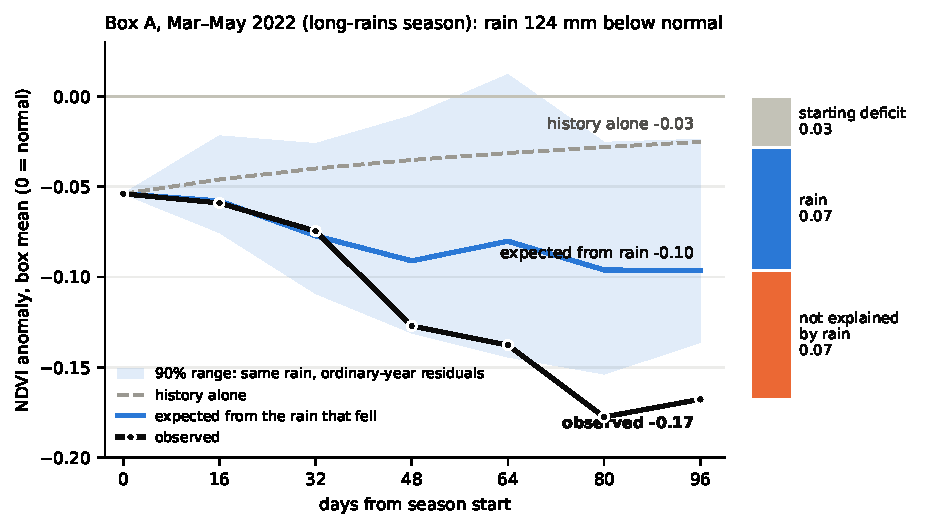
\includegraphics[width=\textwidth]{fig_attribution.pdf}
\caption{The 2022 drought, Box A, a held-out year, box means. Grey dashed: history only, the incumbents' baseline. Blue: what the learned model expects from the rain that fell, residual set to zero. Black: observed. Shading: $90\%$ range of the same rollout with ordinary-year residuals re-injected (Appendix). Right: the season-end anomaly split into the deficit the season began with, the rain's share (observed minus the counterfactual of \eqref{eq:cf} under normal rain), and the residual (observed minus blue). History says recovery, the model says half the fall, the land fell further.}
\label{fig:attribution}
\end{figure*}

\paragraph{Fit} M2's one-step skill exceeds M1's by $0.07$ on unseen years and $0.05$ on the unseen landscape, and its spread is calibrated (Appendix). Along the rain that fell, three-month error is $23\%$ below history and $13\%$ below the S-curve on unseen years, $17\%$ and $8\%$ on the unseen landscape (Figure~\ref{fig:response}, Table~\ref{tab:onestep}). Fed climatological rain the same network falls behind history within two months; fitted without rain its skill is $0.016$. The S-curve's amplitude fitted near zero: the nonlinearity is in how rain interacts with pixel, state and season, not in rain alone.

\paragraph{Residual and counterfactual} In October--December 2020 rain was $38$\,mm below normal and the counterfactual ends within $0.05$ NDVI of the observation: near-normal rain, near-zero rain effect. In March--May 2022 rain was $124$\,mm below normal: the box ended $0.17$ NDVI below normal (Figure~\ref{fig:attribution}). History alone predicts recovery, so a z-score assigns the whole $0.17$ to the land. The model assigns $0.07$ to the rain that failed, $0.07$ to the residual, and the rest to the deficit the season began with; under normal rain with the residual held fixed the land ends $0.10$ below. That normal-rain run is the baseline for a credit; observed minus it is the rain's share, the quantity an index insurer pays on. The land leaves the range of ordinary non-rain variation only in the last month of the season, and history's recovery sits at that range's upper edge. Where rain is more than $60$\,mm below normal the residual is systematically negative: part of the 2022 residual is model under-response to a drought deeper than its training. Read as a likelihood, the same residual tells drought from disturbance: with every score tuned to flag $5\%$ of unburned land, the two drought seasons draw $24\%$ false alarms from a z-score and $5\%$ from the model (Table~\ref{tab:anomaly}). Scoring the residual against mapped burns is out of scope here; protocol, figure and full results are in the Appendix (Figure~\ref{fig:fire}).

\paragraph{Sensitivities}
\begin{table*}[t]\centering\footnotesize\setlength{\tabcolsep}{3pt}
\caption{Does $\Delta$ rank patches by their real response to rain? Held-out rainy-season steps 2019--25, in thirds by M2's $\Delta$ at the starting state, split at each box's median rain departure. Response: NDVI change two steps on per $100$\,mm of rain anomaly, given starting greenness; $\pm$ two bootstrap s.d.; bold clears zero.}\label{tab:greeks}
\begin{tabular}{llccccc}\toprule
 & Rain & \multicolumn{3}{c}{Real response, by $\Delta$ third} & Model $\Delta$ & Most $-$\\
Landscape & departure & least & medium & most & by third & least\\\midrule
A, unseen years & $\le 30$\,mm & $.096\pm.092$ & $.088\pm.100$ & $.147\pm.096$ & $.041/.087/.124$ & $.051\pm.160$\\
 & $> 30$\,mm & $.034\pm.018$ & $.066\pm.034$ & $.078\pm.038$ & $.032/.088/.123$ & $\mathbf{.044\pm.040}$\\
B, unseen land & $\le 21$\,mm & $.083\pm.066$ & $.286\pm.238$ & $.237\pm.140$ & $.064/.097/.122$ & $\mathbf{.154\pm.135}$\\
 & $> 21$\,mm & $.062\pm.042$ & $.087\pm.048$ & $.131\pm.034$ & $.066/.098/.123$ & $\mathbf{.070\pm.051}$\\\bottomrule
\end{tabular}
\end{table*}

\textbf{$\Delta$ -- } On the grid mean an extra $100$\,mm of rain in March--May raises greenness by a (mean) peak of $0.075$ NDVI a month later, positive in sign at every pixel and half gone by three months ($.029/.075/.073/.060/.047/.036$ by 16-day step). Recomputed from the current state at each rainy-season step, $\Delta$ sorts exposure well. Sorted by $\Delta$, the top third of patches green about twice as much per $100$\,mm as the least, on unseen years and landscape, with the right magnitudes on that landscape (Table~\ref{tab:greeks}). We also find that the response is a property of the pixel's state, not of the pixel: a frozen map averaged over the training years is no better than a single constant (Table~\ref{tab:greekstests}), and its rank correlation with the real response drops from $0.70$ to $0.38$ frozen on Box A.

\textbf{$\Theta$ -- } A measure of impact decay over time, the $\Theta$ produced here predicts the impact of exogenous shock halves in $35$ days in the long rains and $38$ in the dry, against $38$ days in the anomaly's raw autocorrelation (Figure~\ref{fig:greeks}).

\textbf{$\partial\sigma/\partial r$ -- } The model predicts both a spread $\sigma$ and a mean $\mu$. An extra $100$\,mm widens the one-step spread by a mean average of $21\%$ on Box A and $32\%$ on the unseen landscape, at every pixel individually. Held-out steps bear it out: sorted by the rain that fell, predicted spread rises from $.060$ to $.082$ as realised error rises from $.061$ to $.093$, although the model in its current configuration still under-predicts spread through the middle of that range. Black--Scholes has no equivalent because it assumes $\sigma$ constant -- the volatility smile \citep{rubinstein1994,dupire1994} is an artifact of this assumption's limitation.

\section{Conclusion}
Inverting our learned transition density world model on observed satellite data produces the residual, what the land did beyond the rain's effect. By differentiation, it returns key sensitivities --- what a pixel's greenness is attributable to, how long a shock to it lasts, and how much rain widens the range of outcomes. Read as a likelihood, it tells drought from exogenous disturbance. In March--May 2022, a held-out year, Box A ended $0.17$ NDVI below normal. The model accounts $0.07$ to the rain that failed, and re-run under normal rain with the residual held fixed the land still ends $0.10$ below, representing a baseline a credit or a payout should be measured against (Figure~\ref{fig:attribution}). A z-score would predict recovery that season and attribute the whole $0.17$ to management. While only a proof of concept on limited data and with various simplifications, we believe this invertible transition density approach has real potential to practical world modelling of complex real-world temporal systems that has genuine utility.

\bibliography{references}
\end{document}
